\chapter{Introducción}\label{cap.introduccion}
\hspace{1cm} En este primer capítulo, antes de adentrarnos en la parte mas técnica, se va a introducir al lector de forma breve en qué es la robótica y más concretamente en los robots aéreos, para así conocer el estado actual de este campo y cómo ha evolucionado en los últimos años este sector, creando una gran rama dentro del mundo de la aviación. Este TFG presenta un robot aéreo que utiliza visión para navegar por lo que comentaremos también ese contexto en el que se encuadra.

\section{Robótica actual}
\hspace{1cm} La Robótica es una rama multidisciplinar de la ingeniería y la ciencia la cual incluye partes de la ingeniería mecánica, ingeniería eléctrica, ciencias de la computación y otras. Estas tecnologías permiten desarrollar máquinas que puedan sustituir a los humanos en sus acciones más cotidianas.Sobretodo están pensadas para ser usadas en ambientes peligrosos (detección y desactivación de bombas), procesos de manufactura (montaje en serie de coches) e incluso en ambientes donde los humanos no pueden sobrevivir (otros planetas como Marte).

\hspace{1cm} Los principios básicos, que se plantearon por Isaac Asimov, para el correcto funcionamiento de los robots fueron: primero, que ningún robot puede hacer daño a un ser humano, o permitir que se le haga daño por no actuar; segundo, que un robot debe obedecer las órdenes dadas por un ser humano, excepto si estas órdenes entran en conflicto con la primera ley; y tercero, que un robot debe proteger su propia existencia en la medida en que está protección no sea incompatible con las leyes anteriores. Todo esto actualmente  dista mucho de la realidad y, aunque sí que se exigen unos mínimos a la hora de crear robots, cualquier parecido con la robótica de ciencia ficción en las películas es mera casualidad.
\\
\\
\begin{figure}[H]
 \centering
  \subfloat[Robot Artificiero]{
   \label{f:Robot Artificiero}
    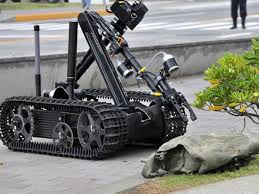
\includegraphics[width=0.33\textwidth]{imag/IMG1.jpeg}}
  \subfloat[Robots en cadena de montaje]{
   \label{f:Robots en serie de montaje}
    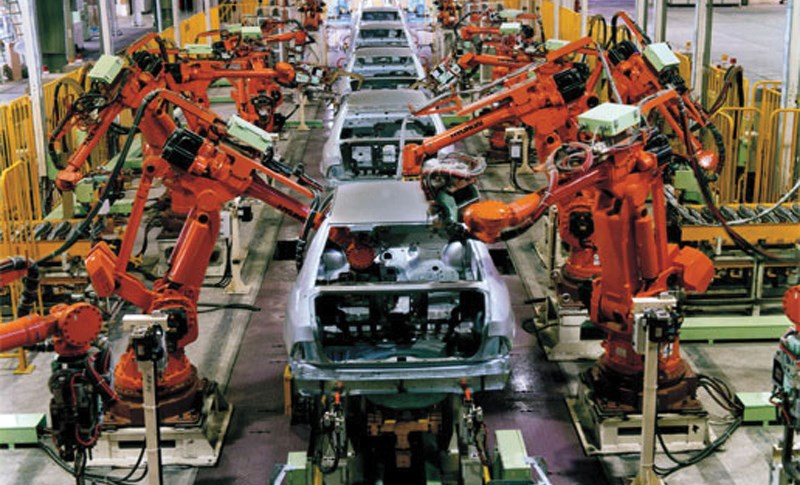
\includegraphics[width=0.33\textwidth]{imag/IMG2.jpeg}} 
  \subfloat[Rover Curiosity en Marte]{
   \newline\label{f:Rover Curiosity en Marte}
    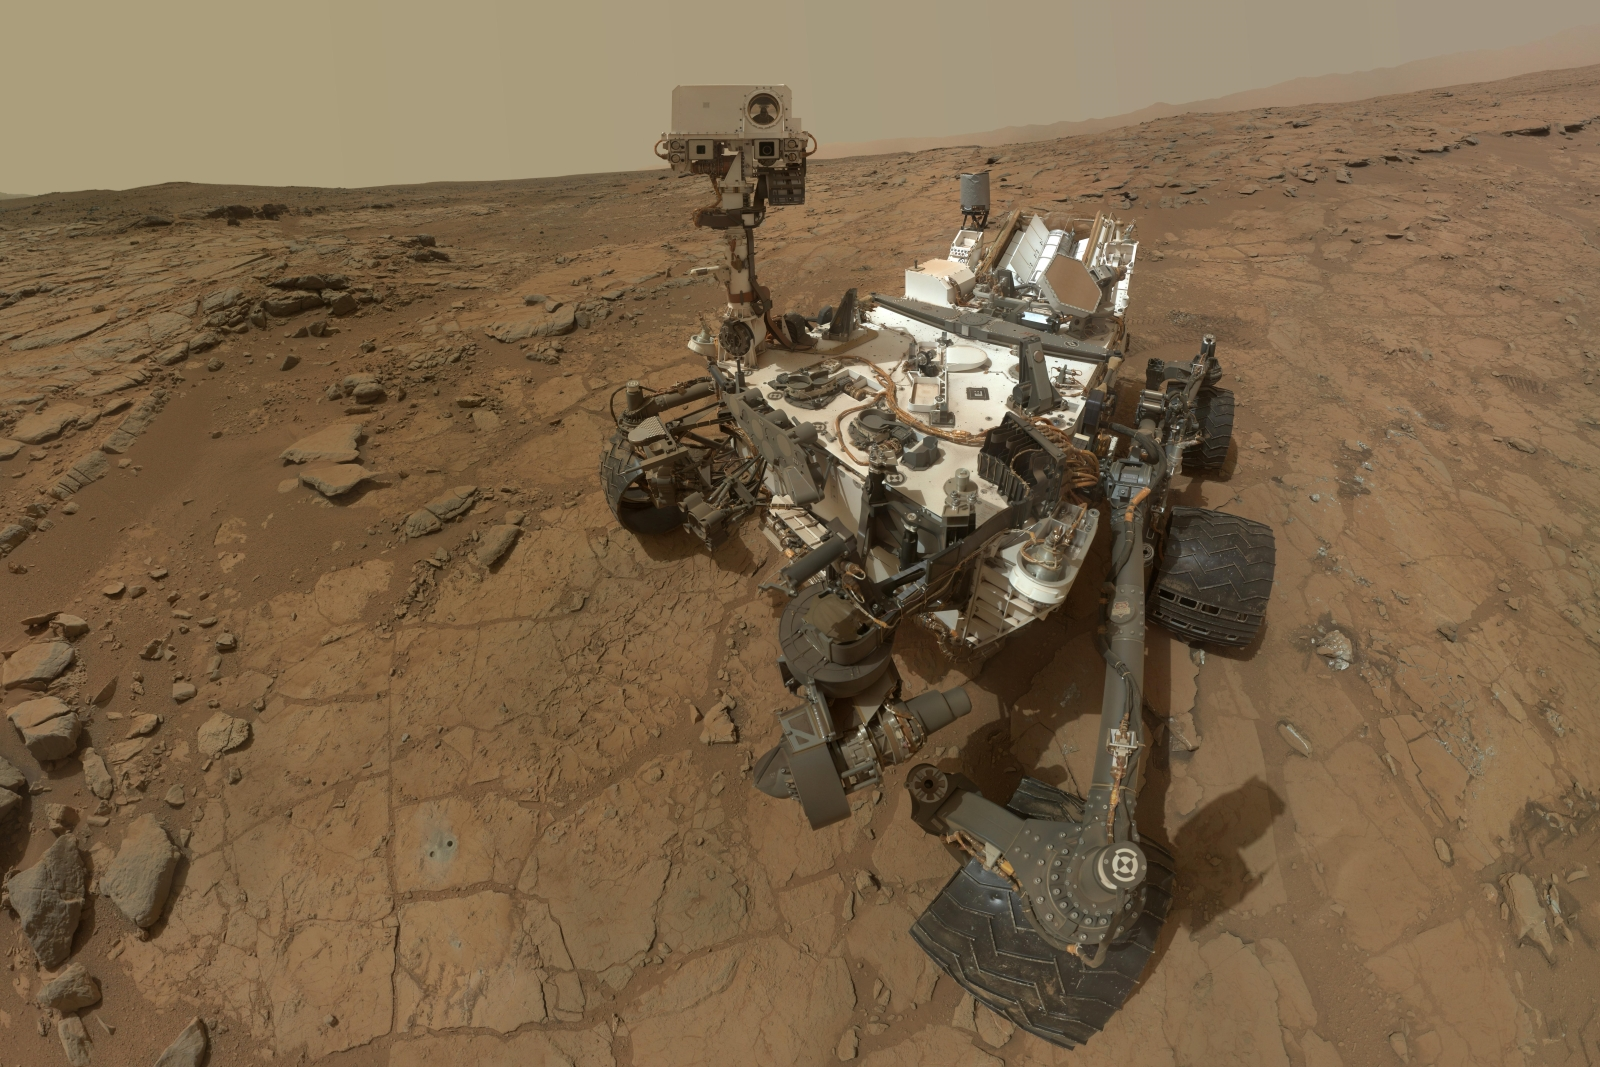
\includegraphics[width=0.33\textwidth]{imag/IMG3.jpeg}} 
 \caption{Ejemplos de funcionalidades de robots}
 \label{f:Ejemplos de funcionalidades de robots}
\end{figure}  

\subsection{Clasificación}
\hspace{1cm} Hay muchas clasificaciones posibles de los robots, uno, bastante utilizado, y reconocido, es según su cronología:

\begin{itemize}
		\item \textbf{1ª Generación:} Robots manipuladores. Sistemas mecánicos de varias funcionalidades con un sistema de control sencillo, el cual puede ser manual, de secuencia fija o de secuencia variable.

	\item\textbf{2ª Generación:} Robots de aprendizaje. Son capaces de repetir una secuencia de movimiento que ha sido previamente ejecutada por una persona. El operador realiza los movimientos requeridos mientras el robot los memoriza y le va siguiendo. 

	\item\textbf{3ª Generación:} Robots con control sensorizado. Llevan incorporados controladores, pequeñas computadoras que ejecutan las órdenes de un programa y es capaz de realizar los movimientos ordenados.

	\item\textbf{4ª Generación:} Robots inteligentes. Similares a la generación anterior pero incluyen una gran mejora, están equipados con sensores que mediante la comunicación con la computadora de control permite una toma inteligente de decisiones y un control de procesos en tiempo real.
\end{itemize}

\begin{figure}[H]
	\begin{center}
		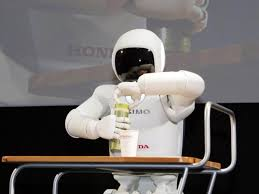
\includegraphics[width=0.5\textwidth]{imag/IMG11.jpeg}
				\caption{Robot ASIMO realizando acciones cotidianas.} 
	\label{fig:Robot ASIMO.}	
	\end{center}
\end{figure}

\subsection{Aplicaciones}
\hspace{1cm} La robótica está en constante desarrollo, esto ligado al incremento de los procesadores, así como en dispositivos hardware y desarrollo de software ha permitido que la robótica esté presente en prácticamente todas las industrias actuales y cotidianas de nuestra vida:
\begin{itemize}
		\item \textbf{Agricultura: }Hoy en día es muy común ver robots que controlen y monitorice por sí solos las cosechas y a medida que pasa el tiempo se vuelven más y más populares. La tecnología robótica aplicada al sector agrícola se encuentra en un estado de desarrollo avanzado debido a la necesidad de aumentar la producción sin aumentar los recursos, al mismo tiempo que se minimiza el impacto ambiental.
		\item \textbf{Educación: }La robótica ha surgido como un recurso didáctico innovador que favorece la enseñanza de conceptos y conocimientos de distintas disciplinas, no únicamente las tecnológicas o científicas.  Además, esta tecnología  se utiliza como factor de motivación, a partir del interés de los niños, para llevar al alumno al desarrollo de su propio conocimiento.
\\
		\begin{figure}[H]
			\begin{center}
				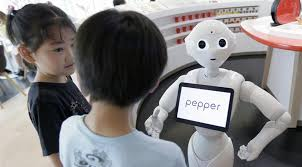
\includegraphics[width=0.9\textwidth]{imag/IMG12.jpeg}
					\caption{Robot PEPPER en un aula como complemento educador.}
			\label{fig:Robot PEPPER.}	
			\end{center}
		\end{figure}

		\item \textbf{Industria: }Se utilizan para realizar trabajos peligrosos o de gran dificultad para un humano, como puede ser la aplicación de sustancias nocivas, el moldeado de materiales o el transporte pesado; también para tareas de inspección y control de calidad mediante visión artificial y sistemas mecánicos. Además, el uso de robots conlleva una mejora de calidad y un gran aumento de la productividad, por ejemplo ayudando a la logística y el procesado final para los envíos.
		\item \textbf{Automovilismo: }En las fábricas se utilizan para ayudar en la fabricación, como los brazos robóticos de montaje o para el transporte de materiales, como los AGVs que son capaces de guiarse por la fábrica autónomamente. Fuera de éstas podemos observar vehículos con conducción autónoma que poco a poco son cada vez más utilizados, como Tesla, BMW y los sistemas de aparcamiento autónomo. También en la investigación espacial se hace un gran uso de la robótica, lo que permite investigar entornos que para un ser humano serían prácticamente imposibles, como el caso del robot Curiosity.
		\item \textbf{Medicina: }Se han desarrollado dispositivos que permiten realizar desde trabajos quirúrgicos guiados por imágenes hasta cirugía mínimamente invasiva realizada mecánicamente por un robot. Es el caso del robot DaVinci, capaz de realizar operaciones por sí solo con un nivel de precisión imposible de alcanzar por un humano y una gran velocidad. También podemos encontrar robots asistenciales para personas que necesitan una supervisión y cuidado continuo, prótesis robóticas para sustitución parcial de alguna parte dañada del cuerpo, o incluso exoesqueletos. Otro ejemplo estaría en la robótica terapéutica, utilizada como medio de rehabilitación fisiológica y de estimulación cognitiva en tratamientos para enfermedades como el Alzheimer.
		
		\begin{figure}[H]
			\begin{center}
				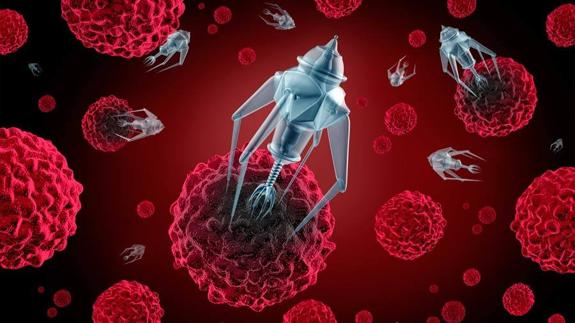
\includegraphics[width=0.54\textwidth]{imag/IMG13.jpeg}
					\caption{Robot DaVinci utilizado en hospitales.}
			\label{fig:Robot DaVinci.}	
			\end{center}
		\end{figure}	
			
		\item \textbf{Militar: } Actualmente existe una gran gama de vehículos terrestres sin piloto humano con funciones de reconocimiento e incluso algunos vehículos armados. Un ejemplo de esto sería el robot PackBot que según el medio en el que se encuentre se puede equipar con diferentes instrumentos para adaptarse a el. El mayor desarrollo en cuanto a robótica militar está siendo en la robótica aérea, donde estos sistemas han pasado de ser unidades de apoyo a unidades primarias de ataque.
		\item \textbf{Ocio y tiempo libre: }En los últimos años se ha producido una integración de esta tecnología en eventos de cultura, deporte y ocio e incluso en las casas. En las casas donde podemos ver robots autónomos que se encargan de las tareas domésticas como la aspiradora Roomba. Aquí también podríamos incluir los robots para niños que son capaces de divertir y entretener a la vez, y están llegando a todos los hogares, los más vendidos son los robots de LEGO donde los niños pueden aprender a crear robots y programarlos de una forma muy sencilla. Por último mencionaremos el robot que está creando gran expectación por sus habilidades locomotrices y aspecto humanoide, es el llamado Atlas creado por Boston Dynamics, capaz de correr y saltar en cualquier tipo de entorno e incluso de dar volteretas.
				
		\begin{figure}[H]
			\begin{center}
				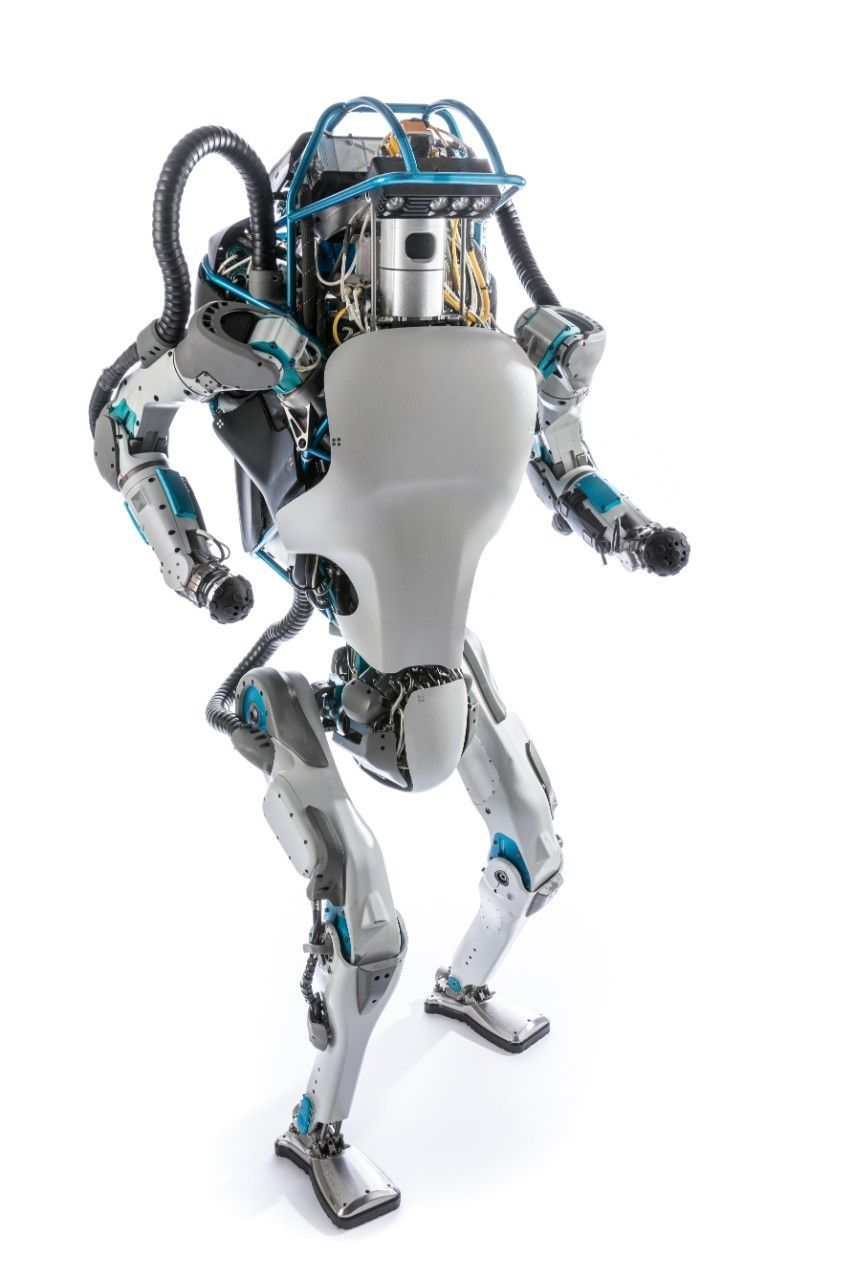
\includegraphics[width=0.25\textwidth]{imag/IMG29.jpg}
					\caption{Robot Atlas de aspecto humanoide.}
			\label{fig:Robot Atlas.}	
			\end{center}
		\end{figure}
		
		\item \textbf{Seguridad: }La robótica ha dado al mundo de la seguridad y la vigilancia una nueva perspectiva, siendo la visión artificial el eje en torno al que giran estas aplicaciones. La automatización de estas tareas permite una mayor facilidad y eficiencia a la hora de ejecutar esta labor, podemos encontrar drones que vigilan grandes concentraciones de personas, cámaras en seguridad vial que analizan el tráfico o el uso doméstico de estas para la prevención de accidentes.
\end{itemize}

\section{Robótica Aérea}
\hspace{1cm} Los robots aéreos, también conocidos como UAV (\textit{Unmanned Aerial Vehicle}), son vehículos aéreos no tripulados (VANT) controlados remotamente desde una estación de control en tierra y/o mar, o por un programa previamente implementado. Estos últimos son los llamados UAV autónomos, programados para que respondan ante el entorno e incluso interactúen con el.

\hspace{1cm} Inicialmente estos robots se pensaron únicamente para uso militar y fueron desarrollados por este sector. Empezaron a crearse entre los años 1914 y 1918, durante la I Guerra Mundial, como blancos aéreos de entrenamiento y defensa contra los Zeppelins. Se continuaron desarrollando durante la II Guerra Mundial también para entrenar a los operarios de los cañones antiaéreos. Pero pronto se vio el potencial que tenían estos robots aéreos y se empezó a utilizar también con fines más productivos como la vigilancia, iniciada durante la guerra de Vietnam,  y la obtención, manejo y transmisión de información ya sea propia u obtenida por los mismos UAV y así proteger la misma de la guerra electrónica y la criptografía ya que las comunicaciones son mucho más seguras y difíciles de detectar.

\hspace{1cm} Si bien el uso principal en el siglo XX era en la industria militar, en el siglo XXI visto el gran potencial que tenían, los nuevos usos que se les estaban dando y los avances en  la industria aeronáutica e informática hicieron que se convirtiese en una herramienta útil para la sociedad civil. En la actualidad los UAV son útiles en diferentes industrias con diferentes objetivos.

\hspace{1cm} Una posible clasificación de los usos de robots aéreos sería:

\begin{itemize}
		\item \textbf{Blanco:} Servían como simulación de aviones y ataque enemigos para entrenar las defensas de los ejércitos.
		\item\textbf{Reconocimiento:} Uso que reveló el gran potencial de estos robots, servían para enviar información militar recopilada durante el vuelo, normalmente en las zonas enemigas. 
	\begin{figure}[H]
		\begin{center}
			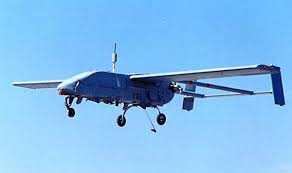
\includegraphics[width=0.7\textwidth]{imag/IMG14.jpeg}
					\caption{AAI RQ-2 Pioneer - Uno de los primeros Robots Aéreos.}
		\label{fig:UAV Pioneer.}	
		\end{center}
	\end{figure}		
		
		\item \textbf{Combate:} estos son los llamados UCAV(\textit{unmanned combat air vehicle}) usados para llevar a cabo misiones de combate que suelen ser peligrosas.
		\item \textbf{Logística:} o también llamados de carga, utilizados sobretodo para transportar mercancías peligrosas o sobre zonas en conflicto sin el riesgo de perder vidas humanas.
		\item \textbf{Investigación y Desarrollo:} en éstos se exploran, prueban y mejoran los sistemas que avanzan cómo serán los drones del futuro.
		\item \textbf{Comercial y Civil:} esta utilización se encuentra en enorme crecimiento tanto de innovaciones como de ventas ya que son diseñados para propósitos civiles como: realizar filmaciones , inspección y reparaciones, sondas de investigación, rescates, vigilancia, detección de incendios y agricultura entre otros.
\end{itemize}

\subsection{Componentes}
\hspace{1cm} La mayoría de los UAV actuales cuentan con una serie de partes, sensores y actuadores que les permiten realizar los propósitos para los que has sido creados, entre ellos se encuentran: 
	\begin{itemize}
		\item \textbf{Motor:} En cuanto a la disposición de los motores diferenciaremos los de ala fija los cuales se rigen por el mismo principio de vuelo que los aviones en los cuales la sustentación se produce gracias a la forma de las alas y el enfrentamiento de estas frente al viento, y los de ala rotatoria, donde los motores giran en horizontal, estos se rigen por el principio de vuelo de los helicópteros en los cuales las propias hélices del motor son las que por su forma y giro producen la sustentación y el vuelo del dron.
		 		
\begin{figure}[H]
 \centering
    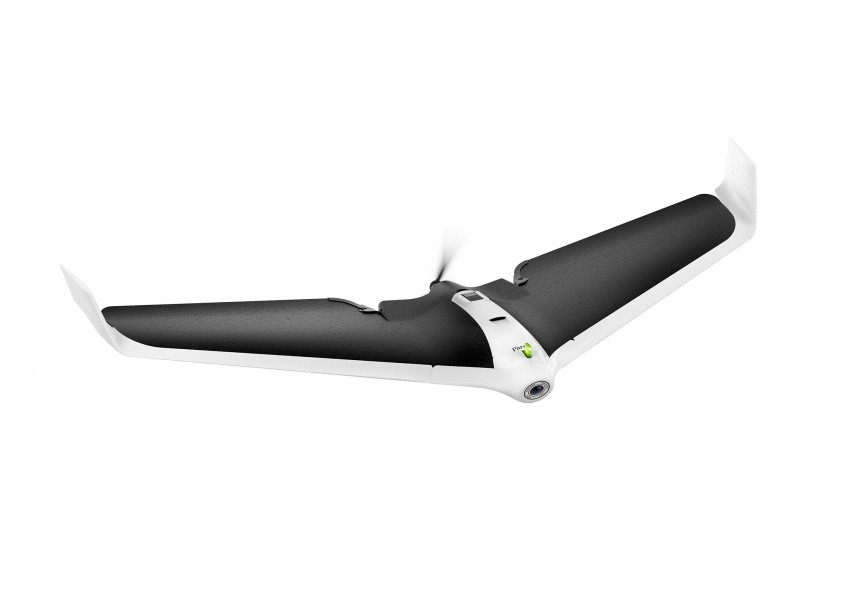
\includegraphics[width=7cm,height=4cm]{imag/IMG15.jpeg}
    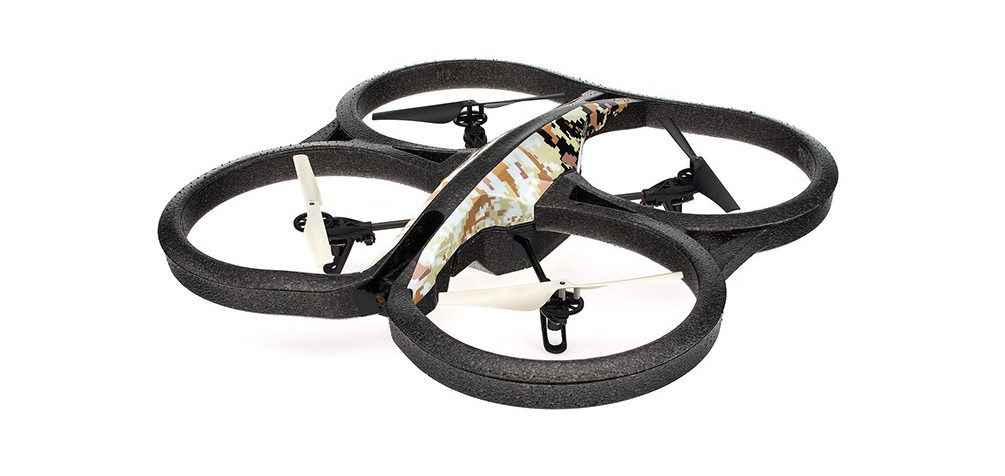
\includegraphics[width=7cm,height=4cm]{imag/IMG16.jpeg}
 \caption{Dron ala fija Vs Dron ala móvil}
 \label{f:Tipos de Dron}
\end{figure}

		\item \textbf{Chasis:} Estructura principal  sobre  la  que  se sitúan el resto de los elementos. Cambiará su forma dependiendo del tipo de UAV, variando la longitud del cuerpo de aterrizaje o el número de soportes para los motores o hélices. Gracias a los últimos avances en la ingeniería de materiales se ha conseguido que el chasis sea muy ligero y con ello incrementar la carga útil (\textit{pay-load}) para mejorar la funcionalidad de los mismos.
		\item \textbf{Batería:} La parte más crítica de los UAV actualmente y en la que más se está investigando. La autonomía media de los UAV no supera la hora de vuelo y esto es debido a que los motores necesitan mucha potencia para poder volar los drones. Cuanto más grande es el dron más potencia es necesaria y por tanto mayor batería se necesita, por lo que hay que encontrar el equilibrio justo que se necesita para cada dron en cuanto a peso, carga útil y autonomía. 
		\item \textbf{Equipo transmisor y receptor:} Parte encargada la transformación de la información y, si fuese el caso, de la comunicación simultánea con el equipo en tierra. Es una parte muy importante para los UAV que están teledirigidos o que transmiten información simultánea de lo que están haciendo, normalmente mediante radiofrecuencia o Wi-Fi.
		\item \textbf{Controlador:} Encargado de recoger toda la información, tanto de la previamente cargada como de los sensores, para procesarla y de ejecutar las órdenes adecuadas para completar el objetivo que se le ha establecido. 
		\item \textbf{Cámara:} Aunque no todos los UAV la llevan incorporada, es una parte imprescindible en el desarrollo de los mismos ya que permite saber en todo momento lo que está realizando el dron y analizar estas imágenes para comprobar el correcto funcionamiento.
		\item \textbf{Altímetro:} Es el sensor que mide los cambios en la presión atmosférica de forma que puede establecer la altura a la que se encuentra el dron.
		\item \textbf{IMU:} es un dispositivo electrónico que mediante una combinación de acelerómetros y giróscopos determina la velocidad, orientación y las fuerzas gravitacionales del vehículo.
		\item \textbf{Magnetómetro:} es un dispositivo que mide la dirección del campo gravitacional de la tierra y de esta forma calcula la orientación del dispositivo con respecto a ésta, lo cual es muy útil para direccionar el dron sobre rutas terrestres.
	\end{itemize}

\subsection{Movimiento de cuadricópteros}
\hspace{1cm} En este TFG nos centraremos sobretodo en los Robots Aéreos de ala móvil, concretamente en los cuadricópteros, que son los que están formados por cuatro hélices las cuales permiten el movimiento en todas las direcciones posibles mediante la variación de potencia de los motores que hacen girar estas hélices. En la imagen \ref{f:Moviento en drones.} se pueden observan cómo se producen los principales movimientos del dron. Las flechas indican el sentido de rotación de las hélices y el color la velocidad del giro, el rojo significa mayor velocidad. Como diferenciación de la forma de vuelo de los helicópteros destacar que en éstos la torsión generada por el rotor principal se contrarresta con una hélice de apoyo perpendicular a ésta y en los drones cuadricópteros el problema de la torsión se solventa asignando el sentido de giro de las hélices de forma opuesta entre rotores que están situados de forma contigua.

\begin{figure}[H]
 \centering
  \subfloat[Rotores en cruz +]{
   \label{f:Rotores en cruz}
    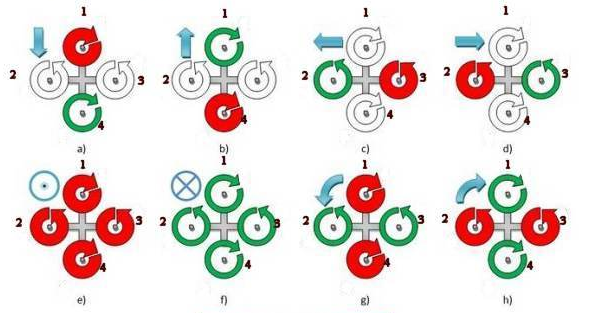
\includegraphics[width=0.53\textwidth]{imag/IMG5.png}}
  \subfloat[Rotores en aspa x]{
   \label{f:Rotores en aspa}
    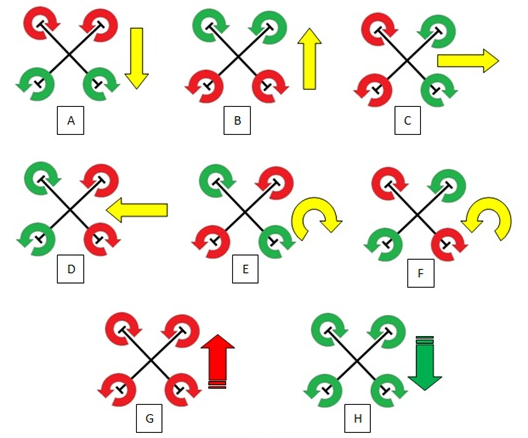
\includegraphics[width=0.38\textwidth]{imag/IMG6.png}} 
 \caption{Movimiento del Dron según sus rotores.}
 \label{f:Moviento en drones.}
\end{figure}

\subsection{Marco legislativo español para drones}
\hspace{1cm} En el marco legislativo actual en España sobre los UAV se acordó el 15 de Diciembre de 2017 en el Consejo de Ministros y se publicó en el BOE \cite{BOE}. La nueva ley sigue cumpliendo prácticamente la totalidad de la ley aprobada el 4 de Julio de 2014 en la cual se especificaba: 
\begin{itemize}
		\item Tipo de Dron: Se establecen dos categorías iniciales: Drones con peso inferior a 2Kg. y drones con peso entre los 2Kg. y 25Kg. Para operar cualquiera de ellos es imprescindible disponer de un carnet de piloto de drones válido en toda España. En caso de los drones de peso inferior a 2kg, no será necesario que estén inscritos en el registro de aeronaves ni disponer de un certificado de aeronavegabilidad. Para ambos tipos de dron será necesario incluir obligatoriamente una placa identificativa con el nombre del fabricante del aparato así como los datos fiscales de la empresa que lleve a cabo dichas operaciones.
		\item Espacio aéreo: El espacio aéreo pertenece a AESA, y como tal, para poder realizar cualquier tipo de actividad comercial o civil con un dron, se deberá obtener un permiso oficial, como mínimo 5 días antes de llevar a cabo cualquier operación en el aire. Esta nueva legislación sigue manteniendo la prohibición de sobrevolar núcleos urbanos o espacios con una alta masificación de gente sin el consentimiento especial por parte de la Agencia Española de Seguridad Aérea.
		\item Seguridad: El pilar fundamental en el que se ha basado el Ministerio para la realización de la normativa de uso de drones civiles en España es la seguridad. Por ello cada empresa deberá disponer de un manual de operaciones cumplimentado siguiendo el estándar proporcionado por el Ministerio, así como un estudio de seguridad de cada una de las operaciones a realizar. Es decir, si alguien piensa en hacer volar un dron al margen de la ley, ya sea con un peso inferior a 2kg, o entre 2kg y 25kg, se expone a sanciones que van entre 3.000\textup{\euro} a 60.000\textup{\euro}.
		\item Carnet de piloto de Drones en España: Para que las empresas puedan operar legalmente los pilotos designados deberán disponer de un carnet oficial para el manejo de drones. Si estos pilotos ya disponen de un título de piloto de avión, ultraligero u otro específico, no será necesario obtener dicha titulación. En caso contrario deberán cursar una serie de exámenes y pruebas oficiales para obtener el carnet oficial de piloto de drones. A día de hoy, no existen academias oficiales bajo la tutela del Gobierno que realicen estos cursos, por eso y mientras se empiezan a impartir estos cursos, será obligatorio demostrar que se dispone de los conocimientos teóricos y algún tipo de carnet oficial o documento que acredite a los pilotos en el manejo de drones para poder llevar a cabo cualquier operación. Esta normativa temporal sobre drones en España considera los diferentes marcos en los que se podrán realizar los distintos trabajos aéreos en función del peso de la aeronave. Además, el texto aprobado se completa con el régimen general de la Ley 48/1960, de 21 de julio, sobre Navegación Aérea, y no sólo marca las pautas de operación con este tipo de aeronaves, sino también otro tipo de obligaciones.
	\end{itemize}
	
\hspace{-1cm} Las únicas novedades de la ley puesta en marcha a finales del año pasado son:

	\begin{itemize}
		\item Sobrevolar zonas pobladas: Ésta es una de las medidas más esperadas por el sector. Se podrán realizar vuelos sobre aglomeraciones, edificios y reuniones de personal al aire libre siempre y cuando la masa máxima al despegue de la aeronave no sobrepase los 10kg, mantengamos la aeronave dentro del alcance visual del piloto (VLOS) y no sobrepasemos los 120 metros de altura ni los 100 metros en horizontal con la posición del piloto.
		\item Vuelos en espacio aéreo controlado: Por el momento sólamente está permitido volar en zonas de espacio aéreo no controlado. Con la nueva ley se podrá volar en espacio aéreo controlado siempre y cuando presentemos los estudios de seguridad correspondiente y tengamos la autorización de AESA.
		\item Operaciones EVLOS: Con la normativa vigente solamente podemos alejar nuestra aeronave a una distancia máxima de 500 metros en horizontal respecto a la posición del piloto. Con la nueva normativa estarán permitidos los vuelos dentro del alcance visual aumentado (EVLOS). Es decir, estos 500 metros pueden ser ampliados, siempre y cuando existan observadores intermedios coordinados entre si. En todo momento, al menos uno de ellos debe tener visión directa del vehículo.
	\end{itemize}	 

\subsection{Competiciones con robots aéreos}
\hspace{1cm} En cuanto a los inventos de drones o de usos de éstos ilustraremos cuatro certámenes importantes. A nivel internacional tenemos el Premio \textit{UAE Drones For Good Award} en los Emiratos Árabes en el cual los siguientes proyectos españoles han llegado a ser finalistas: transferir rápidamente órganos de trasplantes desde los centros de donantes, vigilar mejor las zonas verdes para combatir la caza furtiva, controlar la vida salvaje y reducir el riesgo se incendios, ofrecer mejor detección de campo de minas y combatir la propagación de la enfermedad del sueño (Tse-Tse) mediante el control de mosquitos.

\hspace{1cm} El \textit{UAV Challenge - Outback Rescue} \footnote{\url{https://uavchallenge.org/}} presenta un desafío abierto para adultos y un desafío para la escuela secundaria. El evento tiene como objetivo promover el uso civil de vehículos aéreos no tripulados y el desarrollo de sistemas de bajo costo que podrían usarse para misiones de búsqueda y rescate. Es uno de los desafíos de robótica más grandes del mundo y uno de los desafíos de UAV de mayor riesgo, el premio para el ganador es de 75.000 \$.

\hspace{1cm} Por último a nivel internacional, el certamen más importante de robótica del mundo, el \textit{Mohamed Bin Zayed International Robotics Challenge (MBZIRC)}. La competición está motivada por los desafíos tecnológicos que enfrentan la próxima generación de robótica, ésta está lista para tener un impacto transformador en una variedad de aplicaciones y mercados nuevos, incluyen aplicaciones de robots en respuesta a desastres, petróleo y gas, fabricación, construcción y tareas domésticas. Las tecnologías habilitantes para tales aplicaciones incluyen robots que trabajan de forma más autónoma en entornos dinámicos y no estructurados, mientras colaboran e interactúan con otros robots y humanos. El MBZIRC tiene como objetivo proporcionar un entorno que fomente la innovación y la excelencia técnica, al tiempo que fomenta un rendimiento espectacular con tecnología robótica. El premio para el ganador asciende a 5 millones de dolares.
\\

\hspace{1cm} A nivel nacional tenemos el Premio que se ha creado este año a la Innovación Aeronáutica por el COIAE(Colegio Oficial de Ingenieros Aeronáuticos de España) y que ha ganado un dron que extingue incendios forestales, el cual tiene la capacidad de adaptarse a las condiciones de un fuego para apagarlo \footnote{\url{https://www.drone-hopper.com}}.
\\

\begin{figure}[H]
	\begin{center}
		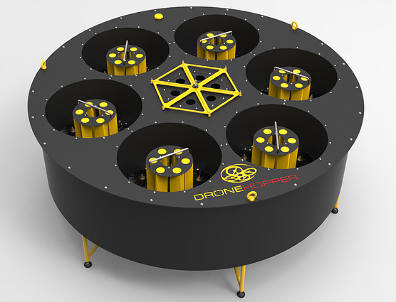
\includegraphics[width=0.7\textwidth]{imag/IMG7.jpeg}
				\caption{Dron contra incendios.} 
	\label{fig:Dron Hopper.}	
	\end{center}
\end{figure}


\section{Visión Artificial y Autolocalización}
\hspace{1cm}  El dron manejado en este TFG incorpora un sistema de autolocalización visual, para muchos científicos el sentido del cual el ser humano obtiene más información del medio es la visión. De hecho, debido a esta gran cantidad de datos se estima que el 70\% de las tareas del cerebro se emplean en analizar estos datos visuales. La visión artificial o visión por computador busca extraer la información visual desde los datos visuales mediante procedimientos automáticos. Para conseguir que esto sea viable y no se tarde días se han desarrollado técnicas de procesamiento de imágenes que han avanzado a niveles de que el desfase entre la visión artificial y la realidad sea prácticamente nulo.

\begin{figure}[H]
	\begin{center}
		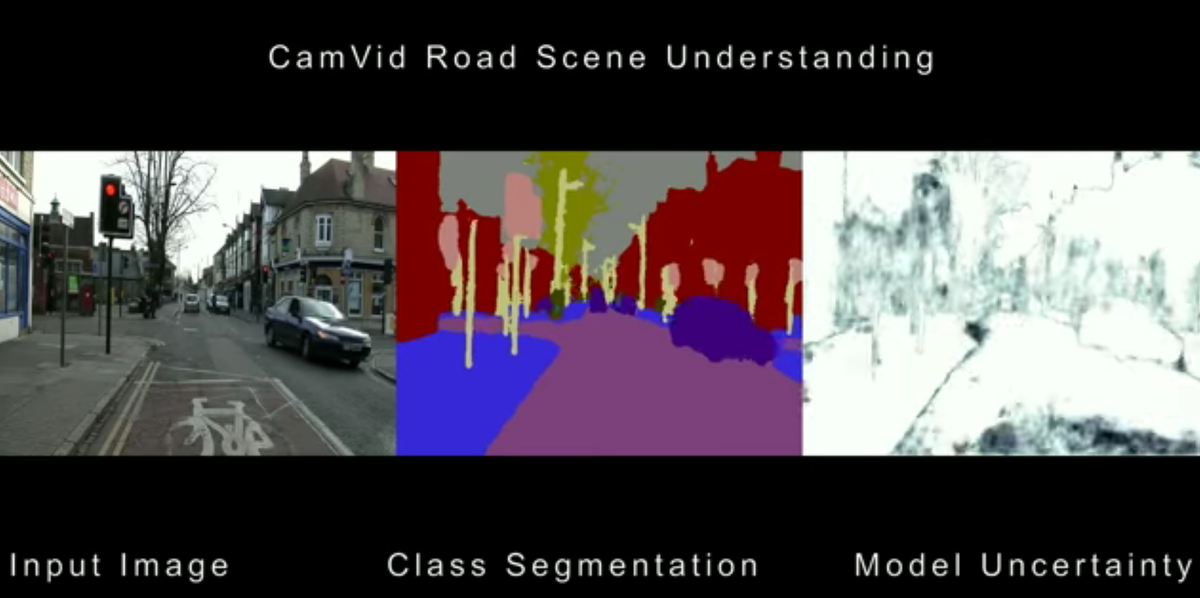
\includegraphics[width=0.9\textwidth]{imag/IMG4.png}
				\caption{Visión artificial de un automóvil.}
	\label{fig:Vista artificial automoviles.}	
	\end{center}
\end{figure}

\hspace{1cm} La visión artificial se basa en la naturaleza de la luz, que es la parte de la radiación electromagnética que puede ser percibida por el ojo humano, está formada por fotones cuyas propiedades en relación con la dualidad de onda explican las características de su comportamiento. La visión artificial se basa en la formación de imágenes y, como hemos dicho antes, en el sistema de procesamiento de éstas. Típicamente el primer apartado de un sistema de visión artificial estaría constituido  por  el  subsistema  de  iluminación,  de  captación  de  la  imagen  y  de adquisición  de  la  señal  en  el  computador. Una vez se ha conseguido introducir la señal en el computador se procesa mediante algoritmos para transformarla en información útil para los robots.

\hspace{1cm} En robótica aérea, especialmente en exteriores, se utilizan sistemas como GPS para la localización de los drones. Sin embargo en interiores no es aplicable ya que no hay cobertura de satélite. Además el sistema satelital tampoco es factible cuando se requiere alta precisión (de centímetros) en el posicionamiento. Por ello, en nuestro proyecto, no podremos utilizar este sistema de posicionamiento y lo cambiaremos por un sistema de autolocalización basado en visión y en balizas, el cual nos dará un error mucho menor y nos permitirá realizar el enrutamiento y guiado mucho más preciso.

\section{Robótica aérea con JdeRobot}
\hspace{1cm} Este TFG se enmarca en el ecosistema del proyecto de software libre para robots JdeRobot. Los antecedentes inmediatos a este TFG en los que me he basado y que me han ayudado para crear mi trabajo han sido:

\hspace{1cm} Alberto Martín \footnote{\url{http://jderobot.org/Amartinflorido-tfm}} \cite{AlbertoMartin} \textit{Navegación visual en un cuadricóptero para el seguimiento de objetos.} En él abordaba la navegación visual autónoma de un cuadricóptero implementando algoritmos de navegación visual para el seguimiento de objetos de manera automática tanto utilizando la cámara frontal como utilizando la cámara inferior.
\\

\begin{figure}[H]
	\begin{center}
		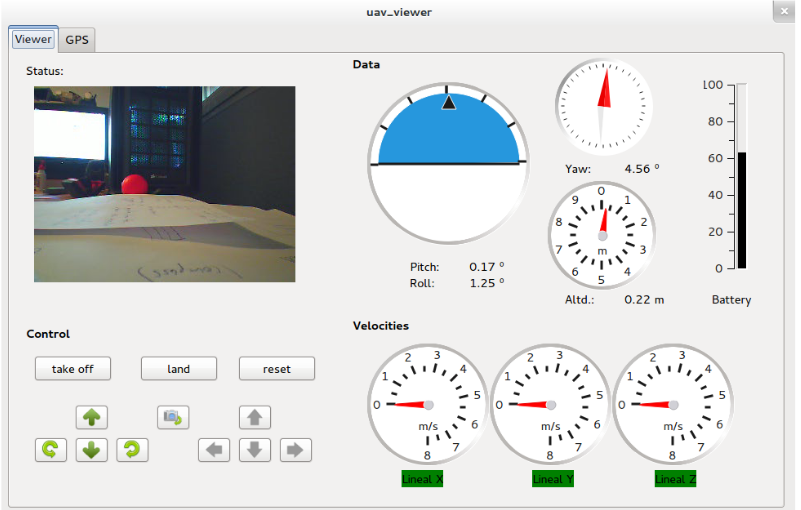
\includegraphics[width=0.8\textwidth]{imag/IMG8.png}
				\caption{TFM Alberto Martín.} 
	\label{fig:TFM Alberto M.}	
	\end{center}
\end{figure}

\hspace{1cm} Daniel Yagüe  \footnote{\url{http://jderobot.org/Daniyague-pfc}} \cite{DanielYague} \textit{Cuadricóptero AR.Drone en Gazebo y JdeRobot}. En el cual su objetivo era proporcionar un soporte para robots aéreos dentro del simulador Gazebo en el entorno JdeRobot y crear varias aplicaciones de navegación para validarlo.
\\

\hspace{1cm} Alberto López-Cerón \footnote{\url{http://jderobot.org/Alopezceron-tfm}} \cite{AlbertoLopez} \textit{Autolocalización visual robusta basada en marcadores.} Su objetivo principal era crear un algoritmo de autolocalización visual basado en marcadores, es decir, a partir de la detección de balizas estimar la posición de la cámara. Fue creado tanto para el entorno de simulación como para entornos reales.
\\

\hspace{1cm} Arturo Vélez \footnote{\url{http://jderobot.org/Avelez-tfg}} \cite{ArturoVelez} Dedicado al \textit{seguimiento de un objeto con textura desde un drone con cámara.} Aquí trabajó en un seguimiento visual, esta vez sin filtro de color, donde el dron sigue una textura en movimiento detectando unos puntos de interés para reconocerla.
\\

\begin{figure}[H]
 \centering
    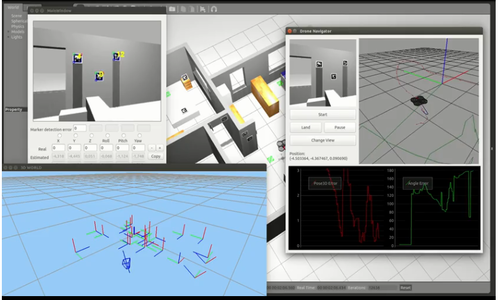
\includegraphics[width=7.6cm,height=6.8cm]{imag/IMG9.png}
    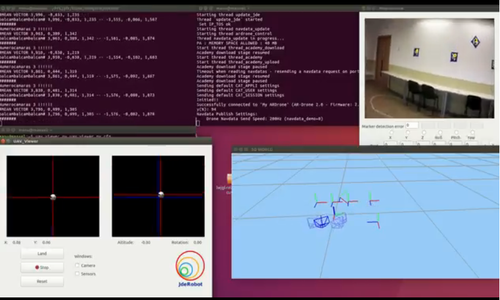
\includegraphics[width=7.6cm,height=6.8cm]{imag/IMG10.png}
 \caption{TFG Manuel Zafra.}
 \label{f:TFG Manuel Zafra}
\end{figure} 

\hspace{1cm} Manuel Zafra \footnote{\url{http://jderobot.org/Mazafrav-pfc}} \cite{ManuelZafra} Centrado en el \textit{seguimiento de rutas 3D por un drone con autolocalización visual con balizas.} Diseñó un sistema de vuelo autónomo para drones en espacios interiores, basándose en la autolocalización mediante la visión artificial como se puede observar en la figura \ref{f:TFG Manuel Zafra}.
\\

\hspace{1cm} Jorge Vela \footnote{\url{http://jderobot.org/Jvela-tfg}} \cite{JorgeVela} Aborda el \textit{despegue, navegación y aterrizaje visuales de un drone usando JdeRobot.} Se centró en la localización y aterrizaje controlado por visión de un dron mediante la detección visual de balizas visible en la figura \ref{f:TFG Jorge Vela}.
\\

\begin{figure}[H]
	\begin{center}
		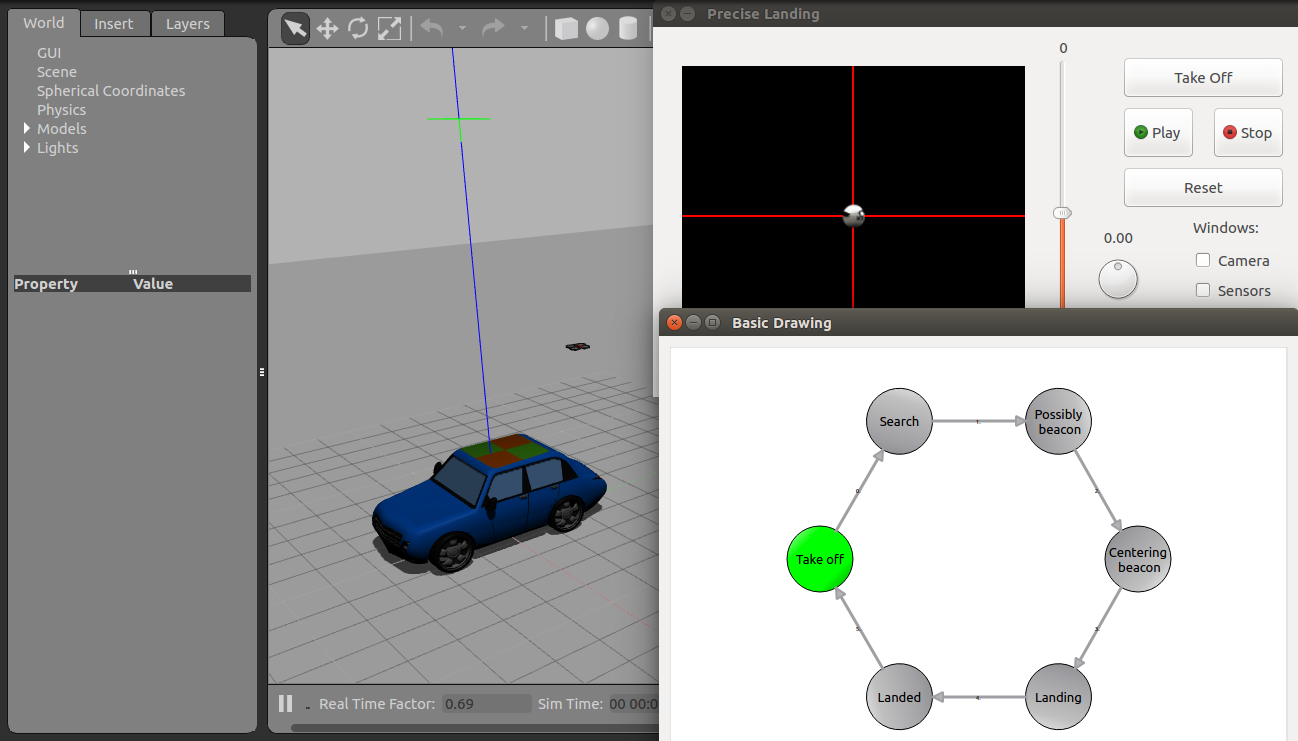
\includegraphics[width=1\textwidth]{imag/IMG50.png}
				\caption{TFG Jorge Vela.}
	\label{f:TFG Jorge Vela}	
	\end{center}
\end{figure}

\hspace{1cm} Una vez expuesta la breve introducción, el resto de la memoria se ha organizado en otros cinco capítulos. En el capítulo 2 se redactan los objetivos propuestos y la metodología seguida para llegar hasta ellos. En el capítulo 3 se presenta la infraestructura que hemos utilizado. En el capítulo 4 se describe el diseño y la implementación del algoritmo realizado, cómo se ha programado y cómo se ha integrado junto con los demás algoritmos en una sola aplicación final. En el capítulo 5 se detallan los distintos experimentos realizados, los resultados y los errores cuantificados que se han obtenido. Por último, en el capítulo 6 se incluyen las conclusiones a las que se han llegado tras finalizar este proyecto y los trabajos futuros que se podrían realizar.
